\chapter[Planificación]{
  \label{chp:plan}
  Planificación
}
\minitoc
\newpage

Neste capítulo explicarase a planificación do traballo realizado e a avaliación de custes.  

\section{Orixe do proxecto}

Produciuse un encontro informal con membros de Cuac FM (a radio comunitaria da Coruña) e a URCM onde se entrou en contacto cos usuarios finais do proxecto a realizar. A URCM (Unión de Radios Comunitarias de Madrid) está composta por unha serie de emisoras independentes e con programas de seu; todos eles listados nunha sección da web (ver figura \ref{fig:urcm}) que á súa vez da acceso ao directorio dos ficheiros de audio (aos que a partir de agora nos referiremos coma \say{audios}) publicados por ditas emisoras. Esta sección da web, pese a súas limitacións, leva funcionando uns anos e resultou ser moi positiva para a redifusión dos programas por distintos colectivos.

\begin{figure}[h]
	\centering
	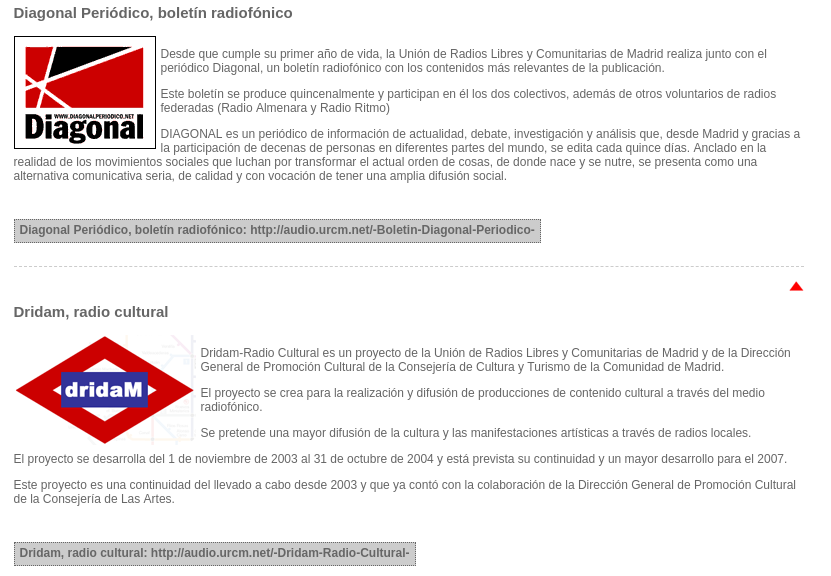
\includegraphics[scale=0.55,keepaspectratio=true]{./images/urcm.png}
	\caption{Sección de audios da web da URCM que inspira o proxecto.}
	\label{fig:urcm}
\end{figure}

Inspirados nesta idea, propúxose crear unha ferramenta semellante, esta vez para a ReMC (Red de medios comunitarios), unha federación de medios comunitarios do Estado Español. Definíronse uns requirimentos iniciais, máis centrados naquel entón na
redifusión e a organización que na escoita.

A seguinte lista é unha transcrición das notas tomadas durante ese encontro:

\begin{itemize}
	\item Os usuarios dos sistema son as propias emisoras.
	\item As emisoras teñen que poder engadir audios.
	\item As emisoras poden acceder aos audios das outras.
	\item As emisoras teñen que poder saber quen está a emitir os seus programas.
\end{itemize}


\section{Iteracións}

Como se explicou no capítulo \ref{chp:metodoloxia}, o desenvolvemento executouse de  de forma iterativa e incremental onde unha iteración son os obxectivos a cumprir entre dúas reunións co cliente. Ao ser isto un proxecto de final de carreira, contarase o tempo entre as sesións de revisión de progresos entre o director do proxecto e o alumno. Estas reunións tiveron unha periodicidade bisemanal na súa meirande parte, reducindo a duración dos ciclos nas derradeiras fases da implementación.


\subsection{Primeira reunión (Iteración 0)}

Na primeira reunión estableceuse a lista de obxectivos xerais do proxecto repasados xa na sección \ref{obxectivos}. Estes supoñen unha aproximación ao problema máis ambiciosa que a idea orixinal de ter un simple directorio web compartido entre emisoras pois ten en conta as necesidades dos ouvintes e a propiedade dos programas por parte dos seus autores e non necesariamente da emisora, cousa bastante común no mundo da radio comunitaria. Foi neste momento cando se tomou a decisión de utilizar Django coma framework de desenvolvemento e PostgreSQL coma sistema de xestión de bases de datos.

Os obxectivos de cara a primeira iteración foron:

\begin{itemize}
	\item Facer un primeiro borrador do deseño do modelo de datos.
	\item Investigar a manipulación de ficheiros RSS utilizando Python. Desde o principio, a consulta dos ficheiros de RSS intuíuse coma o xeito de manter actualizados os programas mais neste momento aínda non se tomara unha decisión firme de como facelo.
\end{itemize}

\subsection{Iteración 1}

Cumpríronse os obxectivos marcados, entregando un deseño preliminar do modelo de datos na data estimada. No diagrama da figura \ref{fig:classold} vese que o modelo aínda era alleo aos requisitos de Django que se explicarán máis adiante no capítulo \ref{chp:disenho} sobre o deseño.

\begin{figure}[h]
	\centering
	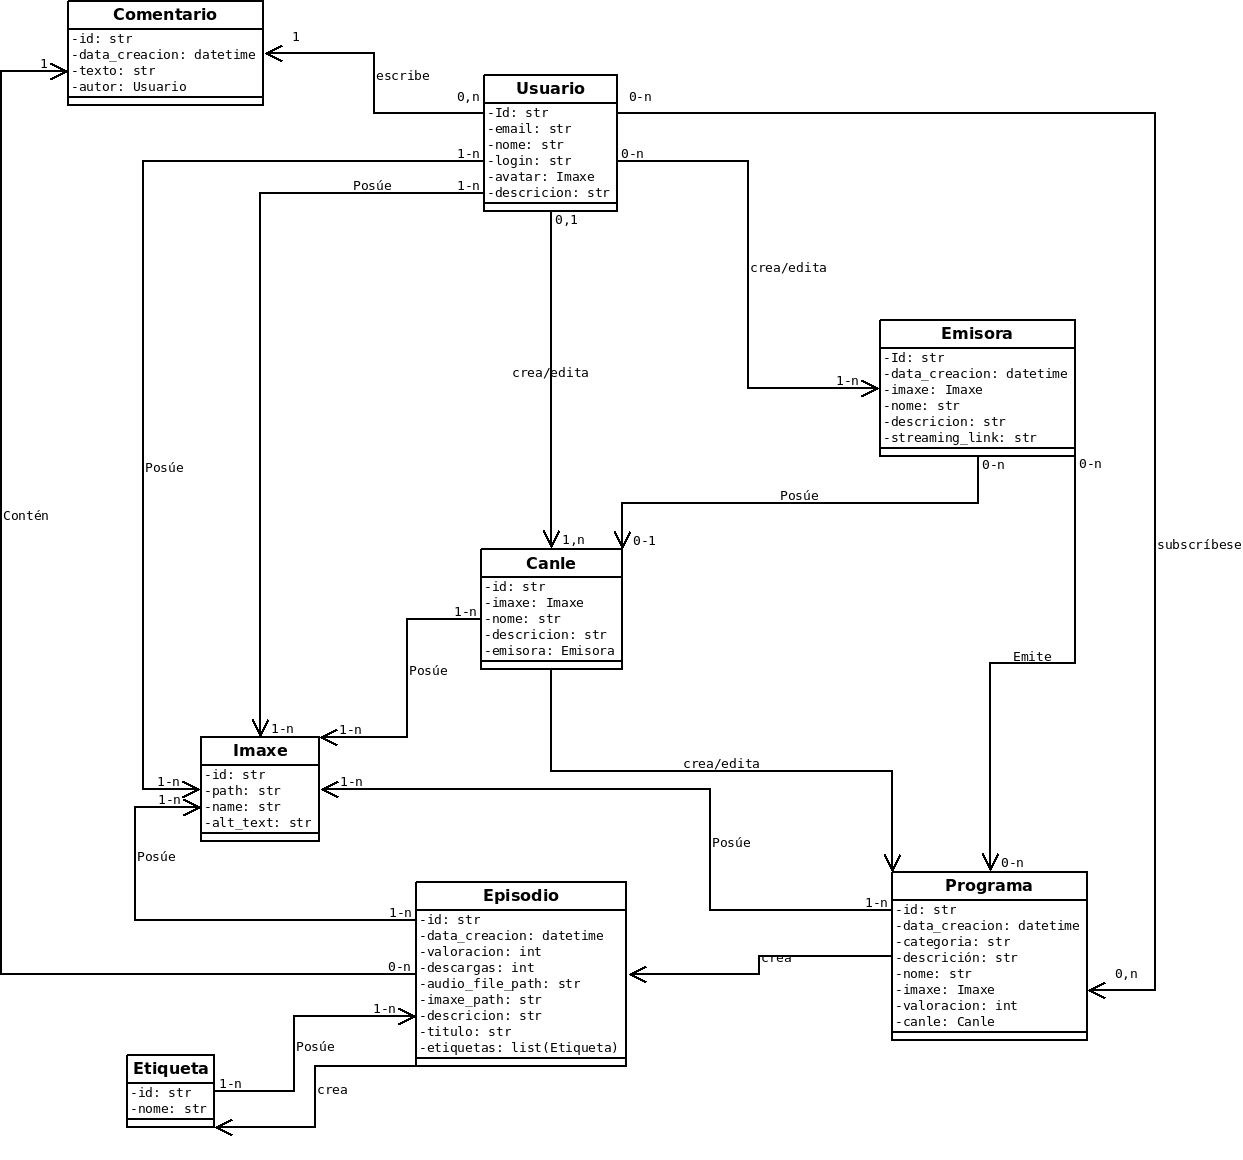
\includegraphics[scale=0.35,keepaspectratio=true]{./images/class_diagram_20171107.png}
	\caption{It1: Diagrama de clases do primeiro borrador de deseño.}
	\label{fig:classold}
\end{figure}

Unha cousa a comentar neste primeiro modelo é a existencia dunha clase \say{canle} intermediaria entre a emisora e o programa que, como veremos, quedou finalmente desbotada. A idea era que os colectivos que realmente teñen unha emisión por onda e aqueles que publican podcasts de escoita baixo demanda terían necesidades distintas e debían diferenciarse, sempre sen bloquear a posibilidade de que unha radio emitise podcasts.

Xa daquela se prevía necesidade de que os usuarios deixasen a súa impresión a cerca dos contidos, expresada no atributo \say{valoración} da clase programa. 

En canto ao RSS, fixéronse os primeiros scripts de proba utilizando a biblioteca de Python \textit{feedparser} incluída no paquete de Anaconda. Ese primeiro código era capaz de descargar un ficheiro RSS e transformalo nun obxecto cos datos do programa que á súa vez contiña unha lista de obxectos cos datos dos episodios, demostrando que a consulta de RSS si era a forma axeitada de afrontar a inserción e actualización dos contidos.

Novos obxectivos:

\begin{itemize}
	\item Instalar a infraestrutura desenvolvemento: Instalación do entorno Django-PostgreSQL.
	\item Implementación de Programa e Episodio.
	\item Implementación dunha interface web básica.
	\item Ampliar o código do script de lectura dos ficheiros RSS.
\end{itemize}

\subsection{Iteración 2}

Ao chegar a seguinte reunión, Django estaba configurado. Creáronse as clases Program e Episode coas súas correspondentes táboas nunha base de datos controlada mediante PostgreSQL. Esas primeiras clases aínda non contiñan información das imaxes nin das etiquetas e os datos non extraíbles do RSS contiñan valores nulos. O sistema executábase sobre o servidor de desenvolvemento de Django, algo que se mantivo durante todo o proceso de desenvolvemento por comodidade e eficiencia. Creouse tamén un repositorio para o control de versións utilizando a plataforma GitHub (ver sección \ref{git})

Conseguiuse a medias o obxectivo de servir unha interface web sinxela: Amosábanse os datos gardados, pero non servía para engadir novo contido aínda. Desprazouse ese obxectivo á seguinte iteración.

\begin{figure}[h]
	\centering
	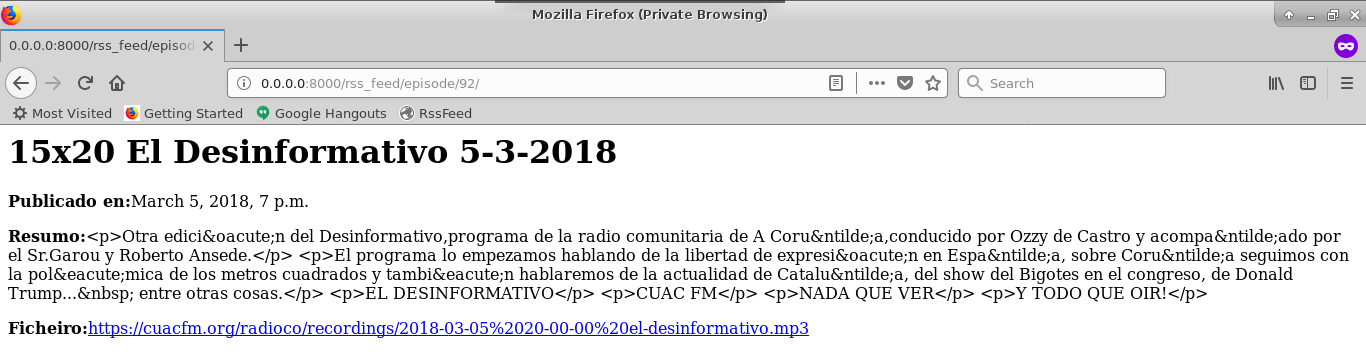
\includegraphics[scale=0.3,keepaspectratio=true]{./images/it2_episode.png}
	\caption{It2: Interface web. Páxina dun episodio.}
	\label{fig:it2_episode}
\end{figure}

Os traballos de ampliación do código de lectura de RSS leváronse a cabo: Os programas e episodios recollían toda a información requirida no momento agás a información de imaxe e de etiqueta (tag). Os traballos neste código revelaron a necesidade de dispor de distintos tipos de lector dependendo da fonte da que o ficheiro RSS fose extraído. 

Novos obxectivos:: 

\begin{itemize}
	\item Engadir formularios á interface para crear novos programas desde ela.
	\item Implementar novos tipos de lector de RSS.
	\item Aplicar \say{plantillas} de estilos ao frontend. 
\end{itemize}

\subsection{Iteración 3}

Nesta iteración creouse o formulario de envío do enlace RSS. Agora, un usuario podía inserir en base de datos o seu programa con todos os seu episodios só con proporcionarlle ao sistema o enlace ao ficheiro. Isto definiu de xeito definitivo o proceso en que os programas e os episodios serían engadidos (non así o aspecto do formulario, que sería cambiado máis adiante).

Instalouse o soporte de Django para Bootstrap 4, podendo así usar eses modelos. Creouse, así, unha páxina de engadir programa co aspecto amosado na figura \ref{fig:it3_add_program}.

\begin{figure}[h]
	\centering
	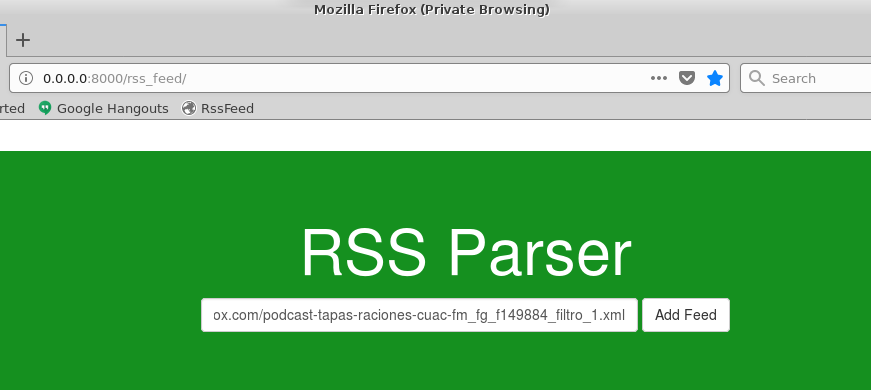
\includegraphics[scale=0.5,keepaspectratio=true]{./images/it3_add_program.png}
	\caption{It3: Interface web. Páxina de engadir programa.}
	\label{fig:it3_add_program}
\end{figure}

Implementouse o soporte para os distintos formatos de ficheiro RSS: Ao principio da iteración só se podían engadir ficheiros extraídos de RadioCo. Ao final, os parsers para Ivoox e Podomatic quedaron tamén implementados. Foi nesta etapa cando se empezou a sentir a necesidade de automatización de probas. Pese a que os 3 tipos de lectores funcionaban, a calidade do código non era a satisfactoria.

Novos obxectivos:

\begin{itemize}
	\item Refactorización dos lectores de RSS.
	\item Implementación das clases de imaxe e etiqueta.
	\item Redefinir a estrutura das páxinas. 
\end{itemize}


\subsection{Iteración 4}

Nesta iteración créase un módulo específico para as funcións de lectura de RSS. Aplícase un patrón estratexia para dar soporte a distintos parsers cunha interface única (máis detalles no capítulo \ref{chp:disenho} sobre o deseño). Para completar o proceso de inserción de programas e episodios, implementáronse as clases da imaxe e etiqueta (Image e Tag).

\begin{figure}[h]
	\centering
	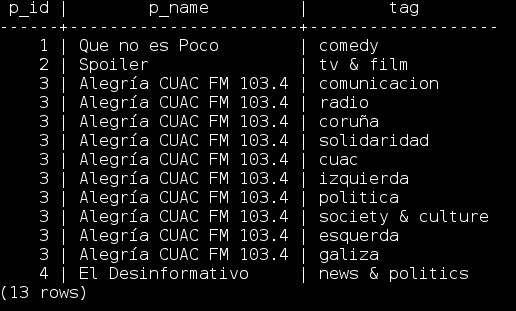
\includegraphics[scale=0.6,keepaspectratio=true]{./images/tags.png}
	\caption{It4: Resultado de consulta á base de datos relacionando programas cos seus tags.}
	\label{fig:it4_tag}
\end{figure}

No tocante á interface, introducíronse nesta iteración as follas de estilo con CSS-Grid, definindo un deseño que serviu coma base do que máis tarde sería o deseño definitivo.

Novos obxectivos:

\begin{itemize}
	\item Crear un proceso que corra no servidor para manter os programas actualizados.
	\item Engadir usuarios ao sistema. 
\end{itemize}

\subsection{Iteración 5}

Levouse a cabo a instalación de Celery e as súas dependencias para correr procesos sobre os seus fíos. Reutilizouse o código do módulo que contén os parsers de RSS. 

No tocante aos usuarios, escribiuse unha primeira versión da autenticación e o rexistro, o cal deu pé a relacionar os usuarios cos seus programas engadidos. Porén, a clase usuario por defecto de Django non satisfacía as necesidades previstas.

Novos obxectivos:

\begin{itemize}
	\item Estender a clase Usuario.
	\item Crear páxina de edición de Ususario.
	\item Facer as vistas dependentes da autenticación.
\end{itemize}

\subsection{Iteración 6}

Introduciuse unha clase de apoio para outorgarlle ao usuario de Django unha serie de atributos necesarios no sistema. Introduciuse a comprobación de autenticación naquelas vistas que o requirisen, por exemplo, engadir programa, como se ve nas figuras \ref{fig:it6_log} e \ref{fig:it6_anon}.

Fíxose unha primeira implementación da vista de edición de usuario, pero sen soporte para o cambio de contrasinal. Quedaría para a iteración seguinte.

\begin{figure}[H]
	\centering
	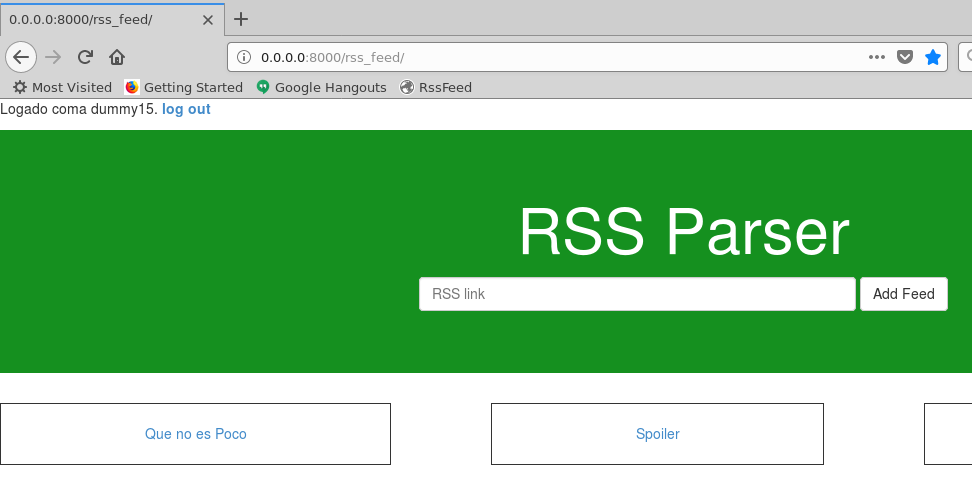
\includegraphics[scale=0.4,keepaspectratio=true]{./images/it6_log.png}
	\caption{It6: index.html para usuario identificado.}
	\label{fig:it6_log}
\end{figure}

\begin{figure}[H]
	\centering
	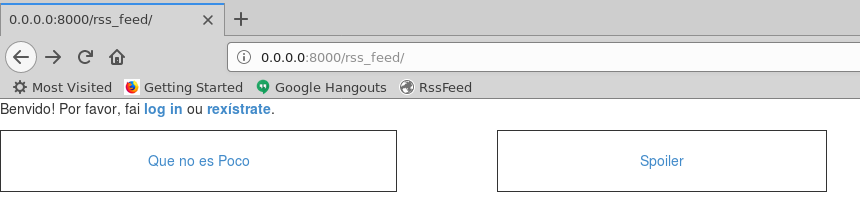
\includegraphics[scale=0.5,keepaspectratio=true]{./images/it6_anon.png}
	\caption{It6: index.html para usuario anónimo.}
	\label{fig:it6_anon}
\end{figure}

Novos obxectivos:
\begin{itemize}
	\item Completar páxina de edición de usuario.
	\item Implementar clases para os votos e os comentarios dos episodios.
	\item Implentar a clase de emisora e canle.
	\item Crear deseño de interacción das páxinas.
\end{itemize}

\subsection{Iteración 7}

Debuxáronse uns deseños esquemáticos das distintas páxinas de interface web e definiuse a navegación entre elas. Este deseño de interface foi xa o definitivo. Valería, en diante, coma guía para confeccionar as distintas vistas.

O resto de obxectivos foron cumpridos. Nesta iteración decidiu desbotarse a clase de Canle por ter unhas funcións moi limitadas e solaparse en gran parte con Emisora.

\begin{itemize}
	\item Dar soporte á internacionalización.
	\item Crear páxina para engadir novas emisoras.
\end{itemize}

